\documentclass[12pt,letterpaper]{article}
\usepackage{graphicx,textcomp}
\usepackage{natbib}
\usepackage{setspace}
\usepackage{fullpage}
\usepackage{color}
\usepackage[reqno]{amsmath}
\usepackage{amsthm}
\usepackage{fancyvrb}
\usepackage{amssymb,enumerate}
\usepackage[all]{xy}
\usepackage{endnotes}
\usepackage{lscape}
\newtheorem{com}{Comment}
\usepackage{float}
\usepackage{hyperref}
\newtheorem{lem} {Lemma}
\newtheorem{prop}{Proposition}
\newtheorem{thm}{Theorem}
\newtheorem{defn}{Definition}
\newtheorem{cor}{Corollary}
\newtheorem{obs}{Observation}
\usepackage[compact]{titlesec}
\usepackage{dcolumn}
\usepackage{tikz}
\usetikzlibrary{arrows}
\usepackage{multirow}
\usepackage{xcolor}
\newcolumntype{.}{D{.}{.}{-1}}
\newcolumntype{d}[1]{D{.}{.}{#1}}
\definecolor{light-gray}{gray}{0.65}
\usepackage{url}
\usepackage{listings}
\usepackage{color}

\definecolor{codegreen}{rgb}{0,0.6,0}
\definecolor{codegray}{rgb}{0.5,0.5,0.5}
\definecolor{codepurple}{rgb}{0.58,0,0.82}
\definecolor{backcolour}{rgb}{0.95,0.95,0.92}

\lstdefinestyle{mystyle}{
	backgroundcolor=\color{backcolour},   
	commentstyle=\color{codegreen},
	keywordstyle=\color{magenta},
	numberstyle=\tiny\color{codegray},
	stringstyle=\color{codepurple},
	basicstyle=\footnotesize,
	breakatwhitespace=false,         
	breaklines=true,                 
	captionpos=b,                    
	keepspaces=true,                 
	numbers=left,                    
	numbersep=5pt,                  
	showspaces=false,                
	showstringspaces=false,
	showtabs=false,                  
	tabsize=2
}
\lstset{style=mystyle}
\newcommand{\Sref}[1]{Section~\ref{#1}}
\newtheorem{hyp}{Hypothesis}

\title{Problem Set 1}
\date{Due: October 1, 2023}
\author{Applied Stats/Quant Methods 1 \\ Dan Zhang 23335541}

\begin{document}
	\maketitle
	
	\section*{Instructions}
	\begin{itemize}
	\item Please show your work! You may lose points by simply writing in the answer. If the problem requires you to execute commands in \texttt{R}, please include the code you used to get your answers. Please also include the \texttt{.R} file that contains your code. If you are not sure if work needs to be shown for a particular problem, please ask.
\item Your homework should be submitted electronically on GitHub.
\item This problem set is due before 23:59 on Sunday October 1, 2023. No late assignments will be accepted.
\item Total available points for this homework is 80.
	\end{itemize}
	
	\vspace{1cm}
	\section*{Question 1 (40 points): Education}

A school counselor was curious about the average of IQ of the students in her school and took a random sample of 25 students' IQ scores. The following is the data set:\\
\vspace{.5cm}

\lstinputlisting[language=R, firstline=37, lastline=37]{PS01.R}  

\vspace{.5cm}

\begin{enumerate}
	\item Find a 90\% confidence interval for the average student IQ in the school.\\
	
	\lstinputlisting[language=R,firstline=40,lastline=52]{PS01.R}
	
	\begin{verbatim}The 90% confidence interval for the average student IQ in the school is :
		[  93.96 , 102.92 ]\end{verbatim}
	
	\item Next, the school counselor was curious  whether  the average student IQ in her school is higher than the average IQ score (100) among all the schools in the country.\\ 
	

	\noindent Using the same sample, conduct the appropriate hypothesis test with $\alpha=0.05$.
	\begin{verbatim}
	step1: Build hypothesis:
  Null hypothesis: The average IQ of school students is equal to the national 
		average IQ.(mu=100)
  Alternative hypothesis: The average IQ of school students is higher than the 
		national average IQ.(mu>100)
	step2:Calculate statistic value by the following code in R
	
	\end{verbatim}
	
		\lstinputlisting[language=R,firstline=56,lastline=69]{PS01.R}
	
	\begin{verbatim}	
		One Sample t-test
		data:  y
		t = -0.59574, df = 24, p-value = 0.7215
		alternative hypothesis: true mean is greater than 100
		95 percent confidence interval: 
		93.95993      Inf
		sample estimates:
		mean of x     
		98.44 
		
		Conclusion:
		As p-value(0.72) is greater than the significance level(0.05). So we can not 
		reject null hypothesis. Which means based on the sample provided,there is no 
		enough evidence to support that the school average IQ socre is higher than the 
		average IQ score in the country.
	\end{verbatim}
	
\end{enumerate}

\newpage

	\section*{Question 2 (40 points): Political Economy}

\noindent Researchers are curious about what affects the amount of money communities spend on addressing homelessness. The following variables constitute our data set about social welfare expenditures in the USA. \\
\vspace{.5cm}


\begin{tabular}{r|l}
	\texttt{State} &\emph{50 states in US} \\
	\texttt{Y} & \emph{per capita expenditure on shelters/housing assistance in state}\\
	\texttt{X1} &\emph{per capita personal income in state} \\
	\texttt{X2} &  \emph{Number of residents per 100,000 that are "financially insecure" in state}\\
	\texttt{X3} &  \emph{Number of people per thousand residing in urban areas in state} \\
	\texttt{Region} &  \emph{1=Northeast, 2= North Central, 3= South, 4=West} \\
\end{tabular}

\vspace{.5cm}
\noindent Explore the \texttt{expenditure} data set and import data into \texttt{R}.
\vspace{.5cm}
\vspace{.5cm}
\begin{itemize}

\item
Please plot the relationships among \emph{Y}, \emph{X1}, \emph{X2}, and \emph{X3}? What are the correlations among them (you just need to describe the graph and the relationships among them)?
\vspace{.5cm}
\lstinputlisting[language=R, firstline=80, lastline=108]{PS01.R}  

\begin{figure}[h!]\centering
		\caption{\footnotesize The relationships between Y/X1/X2/X3 in R.}
		\label{fig:plot_1}
		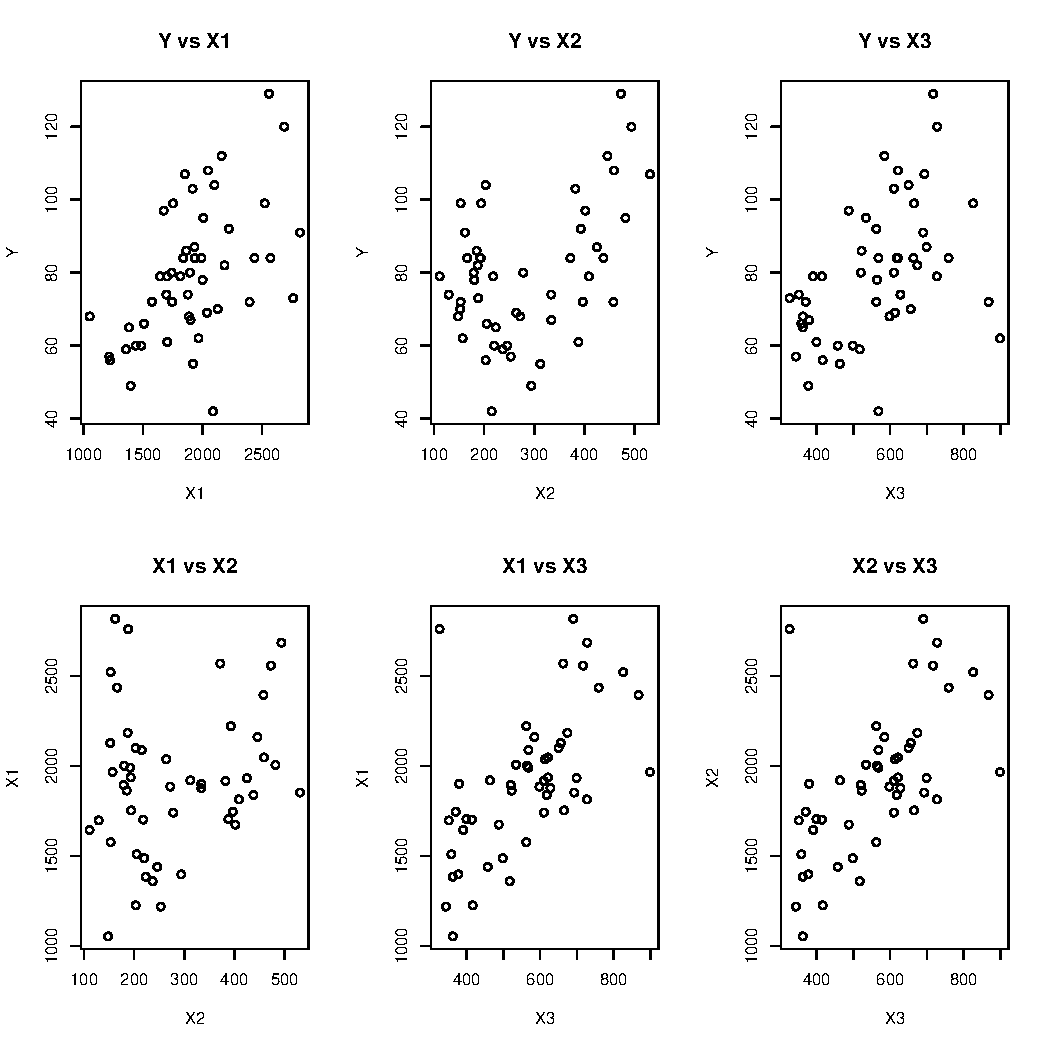
\includegraphics[width=.85\textwidth]{Problem2_Question1_ScatterPlots.pdf}
	\end{figure}

\begin{verbatim}
	Conclusion:
	As we can see from the scatter plots between Y,X1,X2 and X3. There are 
	positive correlations between Y and X1, Y and X3, X1 and X3, X2 and 
	X3,respectively. When the former variable increases, the latter variable 
	also shows an increasing trend. The relationships between X1 and X3, X2 
	and X3, are stronger than the relationships between Y and X1, Y and X3.    
	
	Besides, the correlations between Y and X2, X2 and X2 seem to be 
	non-linear. When X2 is less than about 300, there are negative 
	relationships between Y and X2,X1 and X2. While X2 is greater than 
	about 300, there are positive relationships between Y and X2,X1 and 
	X2.\end{verbatim}
\item
Please plot the relationship between \emph{Y} and \emph{Region}? On average, which region has the highest per capita expenditure on housing assistance?
\vspace{.5cm}
	\lstinputlisting[language=R, firstline=115, lastline=124]{PS01.R}  

	\begin{figure}[h!]\centering
	\caption{\footnotesize The relationships between Y and Region in R.}
	\label{fig:plot_2}
	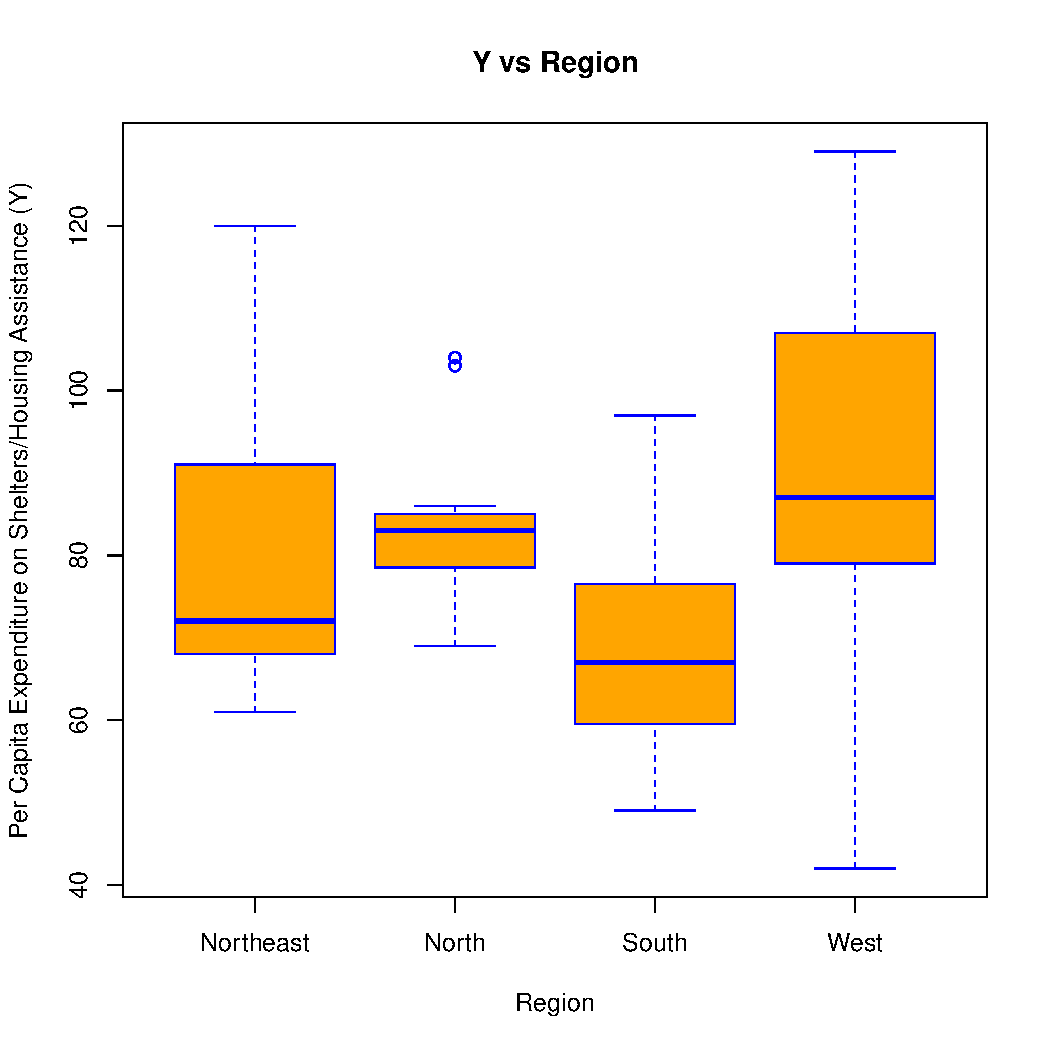
\includegraphics[width=.85\textwidth]{Problem2_Question2_BoxPlot.pdf}
		\end{figure}
		
\newpage

	\begin{verbatim}
	Conclusion:
	According to the boxplot,we can see that region 4 has the highest per 
	capita expenditure on housing assistance.
	\end{verbatim}

\item
Please plot the relationship between \emph{Y} and \emph{X1}? Describe this graph and the relationship. Reproduce the above graph including one more variable \emph{Region} and display different regions with different types of symbols and colors.
\vspace{.5cm}

	\lstinputlisting[language=R, firstline=128, lastline=133]{PS01.R}  

	\begin{figure}[h!]\centering
	\caption{\footnotesize The relationships between Y and X1 in R.}
	\label{fig:plot_3}
	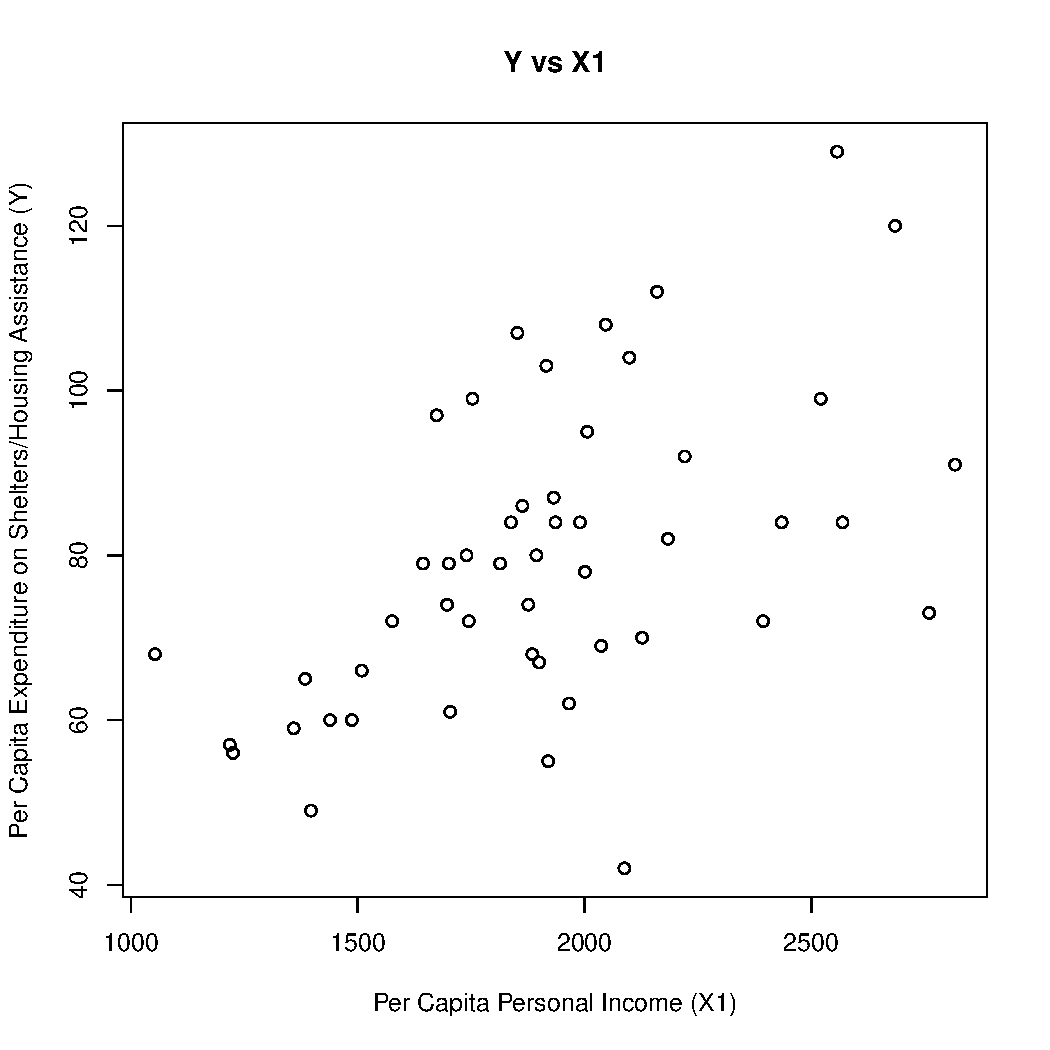
\includegraphics[width=.85\textwidth]{Problem2_Question3_Plot_Y_vs_X1.pdf}
	\end{figure}

	\begin{verbatim}
	As can be observed from the scatter plot, the X-axis represents variable 
	Per Capita Personal Income (X1) and the Y-axis represents variable Per 
	Capita Expenditure on Shelters/Housing Assistance (Y). 
	
	We can see that here is a positive correlation between Y and X1, as X1 
	increases, Y also shows an upward trend. The strength of this relationship 
	is weak and not very close. There might be some sorrelation between Y 
	and X1. Further statistical analysis may help quantify the strength and 
	significance of this relationship.
	\end{verbatim}

	\lstinputlisting[language=R, firstline=139, lastline=160]{PS01.R}  

	\begin{figure}[h!]\centering
	\caption{\footnotesize The relationships between Y X1 and Region in R.}
	\label{fig:plot_4}
	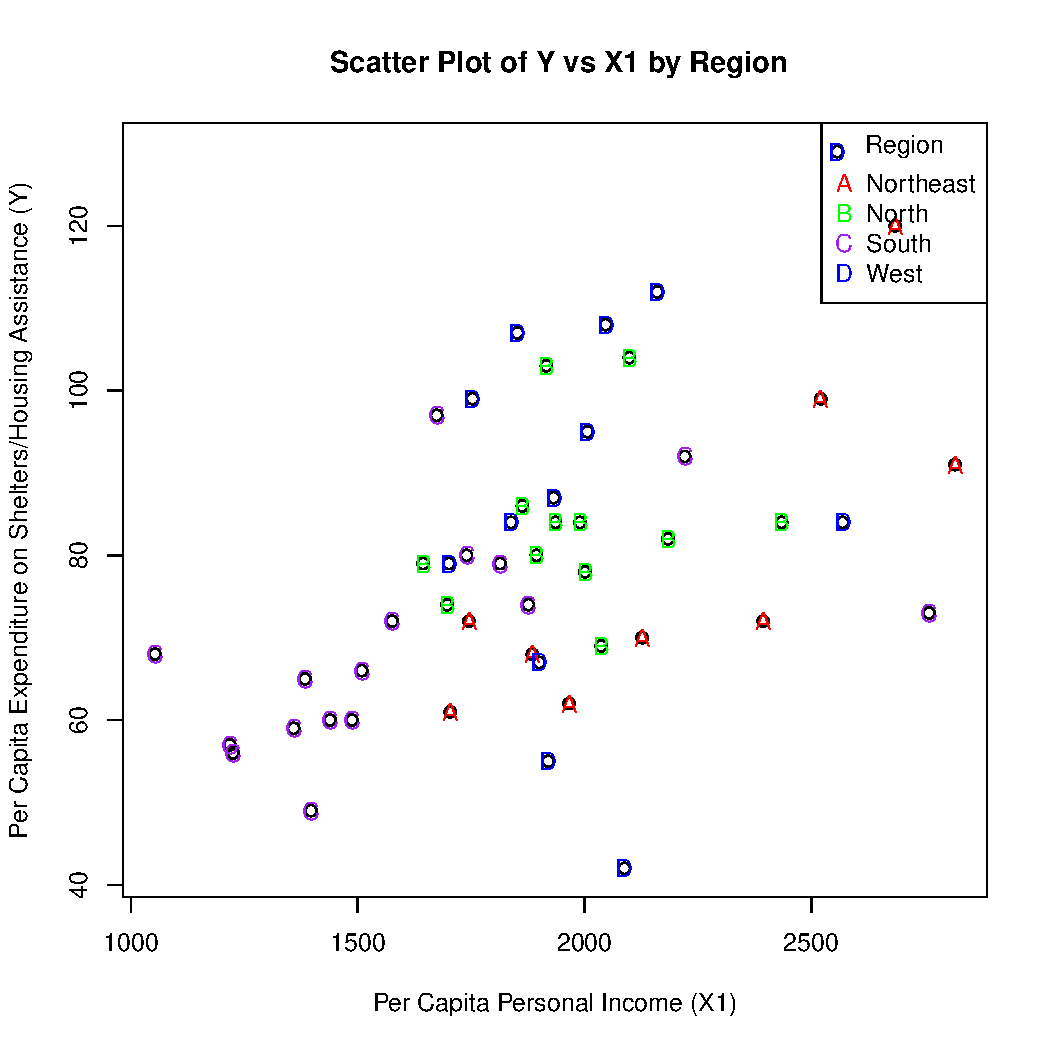
\includegraphics[width=.85\textwidth]{Problem2_Question3_Plot_Y_X1_Region.pdf}
	\end{figure}

\end{itemize}


\end{document}
